\documentclass[]{article}
\usepackage{lmodern}
\usepackage{amssymb,amsmath}
\usepackage{ifxetex,ifluatex}
\usepackage{fixltx2e} % provides \textsubscript
\ifnum 0\ifxetex 1\fi\ifluatex 1\fi=0 % if pdftex
  \usepackage[T1]{fontenc}
  \usepackage[utf8]{inputenc}
\else % if luatex or xelatex
  \ifxetex
    \usepackage{mathspec}
  \else
    \usepackage{fontspec}
  \fi
  \defaultfontfeatures{Ligatures=TeX,Scale=MatchLowercase}
\fi
% use upquote if available, for straight quotes in verbatim environments
\IfFileExists{upquote.sty}{\usepackage{upquote}}{}
% use microtype if available
\IfFileExists{microtype.sty}{%
\usepackage{microtype}
\UseMicrotypeSet[protrusion]{basicmath} % disable protrusion for tt fonts
}{}
\usepackage[margin=1in]{geometry}
\usepackage{hyperref}
\hypersetup{unicode=true,
            pdftitle={Insulin Clamp Study on Mck-TSC1 Mice},
            pdfauthor={Dave Bridges and Nathan Qi},
            pdfborder={0 0 0},
            breaklinks=true}
\urlstyle{same}  % don't use monospace font for urls
\usepackage{color}
\usepackage{fancyvrb}
\newcommand{\VerbBar}{|}
\newcommand{\VERB}{\Verb[commandchars=\\\{\}]}
\DefineVerbatimEnvironment{Highlighting}{Verbatim}{commandchars=\\\{\}}
% Add ',fontsize=\small' for more characters per line
\usepackage{framed}
\definecolor{shadecolor}{RGB}{248,248,248}
\newenvironment{Shaded}{\begin{snugshade}}{\end{snugshade}}
\newcommand{\KeywordTok}[1]{\textcolor[rgb]{0.13,0.29,0.53}{\textbf{#1}}}
\newcommand{\DataTypeTok}[1]{\textcolor[rgb]{0.13,0.29,0.53}{#1}}
\newcommand{\DecValTok}[1]{\textcolor[rgb]{0.00,0.00,0.81}{#1}}
\newcommand{\BaseNTok}[1]{\textcolor[rgb]{0.00,0.00,0.81}{#1}}
\newcommand{\FloatTok}[1]{\textcolor[rgb]{0.00,0.00,0.81}{#1}}
\newcommand{\ConstantTok}[1]{\textcolor[rgb]{0.00,0.00,0.00}{#1}}
\newcommand{\CharTok}[1]{\textcolor[rgb]{0.31,0.60,0.02}{#1}}
\newcommand{\SpecialCharTok}[1]{\textcolor[rgb]{0.00,0.00,0.00}{#1}}
\newcommand{\StringTok}[1]{\textcolor[rgb]{0.31,0.60,0.02}{#1}}
\newcommand{\VerbatimStringTok}[1]{\textcolor[rgb]{0.31,0.60,0.02}{#1}}
\newcommand{\SpecialStringTok}[1]{\textcolor[rgb]{0.31,0.60,0.02}{#1}}
\newcommand{\ImportTok}[1]{#1}
\newcommand{\CommentTok}[1]{\textcolor[rgb]{0.56,0.35,0.01}{\textit{#1}}}
\newcommand{\DocumentationTok}[1]{\textcolor[rgb]{0.56,0.35,0.01}{\textbf{\textit{#1}}}}
\newcommand{\AnnotationTok}[1]{\textcolor[rgb]{0.56,0.35,0.01}{\textbf{\textit{#1}}}}
\newcommand{\CommentVarTok}[1]{\textcolor[rgb]{0.56,0.35,0.01}{\textbf{\textit{#1}}}}
\newcommand{\OtherTok}[1]{\textcolor[rgb]{0.56,0.35,0.01}{#1}}
\newcommand{\FunctionTok}[1]{\textcolor[rgb]{0.00,0.00,0.00}{#1}}
\newcommand{\VariableTok}[1]{\textcolor[rgb]{0.00,0.00,0.00}{#1}}
\newcommand{\ControlFlowTok}[1]{\textcolor[rgb]{0.13,0.29,0.53}{\textbf{#1}}}
\newcommand{\OperatorTok}[1]{\textcolor[rgb]{0.81,0.36,0.00}{\textbf{#1}}}
\newcommand{\BuiltInTok}[1]{#1}
\newcommand{\ExtensionTok}[1]{#1}
\newcommand{\PreprocessorTok}[1]{\textcolor[rgb]{0.56,0.35,0.01}{\textit{#1}}}
\newcommand{\AttributeTok}[1]{\textcolor[rgb]{0.77,0.63,0.00}{#1}}
\newcommand{\RegionMarkerTok}[1]{#1}
\newcommand{\InformationTok}[1]{\textcolor[rgb]{0.56,0.35,0.01}{\textbf{\textit{#1}}}}
\newcommand{\WarningTok}[1]{\textcolor[rgb]{0.56,0.35,0.01}{\textbf{\textit{#1}}}}
\newcommand{\AlertTok}[1]{\textcolor[rgb]{0.94,0.16,0.16}{#1}}
\newcommand{\ErrorTok}[1]{\textcolor[rgb]{0.64,0.00,0.00}{\textbf{#1}}}
\newcommand{\NormalTok}[1]{#1}
\usepackage{longtable,booktabs}
\usepackage{graphicx,grffile}
\makeatletter
\def\maxwidth{\ifdim\Gin@nat@width>\linewidth\linewidth\else\Gin@nat@width\fi}
\def\maxheight{\ifdim\Gin@nat@height>\textheight\textheight\else\Gin@nat@height\fi}
\makeatother
% Scale images if necessary, so that they will not overflow the page
% margins by default, and it is still possible to overwrite the defaults
% using explicit options in \includegraphics[width, height, ...]{}
\setkeys{Gin}{width=\maxwidth,height=\maxheight,keepaspectratio}
\IfFileExists{parskip.sty}{%
\usepackage{parskip}
}{% else
\setlength{\parindent}{0pt}
\setlength{\parskip}{6pt plus 2pt minus 1pt}
}
\setlength{\emergencystretch}{3em}  % prevent overfull lines
\providecommand{\tightlist}{%
  \setlength{\itemsep}{0pt}\setlength{\parskip}{0pt}}
\setcounter{secnumdepth}{5}
% Redefines (sub)paragraphs to behave more like sections
\ifx\paragraph\undefined\else
\let\oldparagraph\paragraph
\renewcommand{\paragraph}[1]{\oldparagraph{#1}\mbox{}}
\fi
\ifx\subparagraph\undefined\else
\let\oldsubparagraph\subparagraph
\renewcommand{\subparagraph}[1]{\oldsubparagraph{#1}\mbox{}}
\fi

%%% Use protect on footnotes to avoid problems with footnotes in titles
\let\rmarkdownfootnote\footnote%
\def\footnote{\protect\rmarkdownfootnote}

%%% Change title format to be more compact
\usepackage{titling}

% Create subtitle command for use in maketitle
\providecommand{\subtitle}[1]{
  \posttitle{
    \begin{center}\large#1\end{center}
    }
}

\setlength{\droptitle}{-2em}

  \title{Insulin Clamp Study on Mck-TSC1 Mice}
    \pretitle{\vspace{\droptitle}\centering\huge}
  \posttitle{\par}
    \author{Dave Bridges and Nathan Qi}
    \preauthor{\centering\large\emph}
  \postauthor{\par}
      \predate{\centering\large\emph}
  \postdate{\par}
    \date{March 21, 2012}


\begin{document}
\maketitle

{
\setcounter{tocdepth}{2}
\tableofcontents
}
\section{Experiment Summary}\label{experiment-summary}

\begin{longtable}[]{@{}llrlrrrrrrrrrrrrrrrrrrrrrrrrrrrrrr@{}}
\caption{All Data}\tabularnewline
\toprule
& Genotype & X. & ID & Basal.Glucose & Clamp.Glucose & Clamp.GIR &
Clamp.AUC & Basal.SA & Clamp.SA & Basal.Gtr & Clamp.Gtr & Basal.HGP &
Clamp.HGP & Basal.sHGP & Clamp.sHGP & Clearance.Basal & Clearance.Clamp
& X0 & X0.1 & X0.2 & X0.3 & Insulin.Basal & Insulin.Clamp & Basal &
Clamp & SOL & TA & Gastroc & V.fat & S.fat & BAT & Heart &
Diaphram\tabularnewline
\midrule
\endfirsthead
\toprule
& Genotype & X. & ID & Basal.Glucose & Clamp.Glucose & Clamp.GIR &
Clamp.AUC & Basal.SA & Clamp.SA & Basal.Gtr & Clamp.Gtr & Basal.HGP &
Clamp.HGP & Basal.sHGP & Clamp.sHGP & Clearance.Basal & Clearance.Clamp
& X0 & X0.1 & X0.2 & X0.3 & Insulin.Basal & Insulin.Clamp & Basal &
Clamp & SOL & TA & Gastroc & V.fat & S.fat & BAT & Heart &
Diaphram\tabularnewline
\midrule
\endhead
8 & Knockout & 8 & 245 & 88 & 113 & 38.3 & 4303 & 166204 & 158722 & 24.1
& 50.9 & 24.1 & 12.56 & 0 & 47.96 & 13.16 & 26.2 & 0 & 0 & 0 & 0 & 1.58
& 21.1 & 0 & 0 & 0 & 0 & 8.32 & 4.880 & 19.05 & 401.6 & 367 &
0\tabularnewline
11 & Knockout & 1 & 266 & 107 & 125 & 40.4 & 4206 & 144050 & 157520 &
33.8 & 62.2 & 33.8 & 21.80 & 0 & 35.48 & 16.87 & 31.2 & 0 & 0 & 0 & 0 &
3.97 & 25.4 & 0 & 0 & 0 & 0 & 17.80 & 13.110 & 22.00 & 95.7 & 262 &
NA\tabularnewline
12 & Knockout & 2 & 267 & 139 & 114 & 14.5 & 1760 & 95930 & 120125 &
50.7 & 82.8 & 50.7 & 68.33 & 0 & -34.65 & 25.60 & 67.1 & 0 & 0 & 0 & 0 &
5.47 & 15.1 & 0 & 0 & 0 & 0 & 11.44 & 4.389 & 25.02 & 172.1 & 348 &
NA\tabularnewline
13 & Knockout & 3 & 323 & 139 & 112 & 15.8 & 1938 & 282602 & 261183 &
16.0 & 34.6 & 16.0 & 18.87 & 0 & -18.31 & 9.34 & 29.2 & 0 & 0 & 0 & 0 &
2.93 & 17.3 & 0 & 0 & 0 & 0 & 17.03 & 5.234 & 17.92 & 112.3 & 405 &
NA\tabularnewline
14 & Knockout & 4 & 371 & 117 & 138 & 31.2 & 3515 & 360233 & 286396 &
14.1 & 38.4 & 14.1 & 7.19 & 0 & 49.18 & 18.20 & 25.9 & 0 & 0 & 0 & 0 &
0.00 & 0.0 & 0 & 0 & 0 & 0 & 21.11 & 8.817 & 32.62 & 322.2 & 440 &
NA\tabularnewline
15 & Knockout & 5 & 197 & 89 & 117 & 31.0 & 3235 & 163434 & 212528 &
30.3 & 46.9 & 30.3 & 15.83 & 0 & 47.77 & 19.92 & 27.8 & 0 & 0 & 0 & 0 &
4.71 & 19.9 & 0 & 0 & 0 & 0 & 16.52 & 4.650 & 39.77 & 120.0 & 405 &
NA\tabularnewline
16 & Knockout & 6 & 184 & 110 & 112 & 25.3 & 2594 & 164238 & 200053 &
29.7 & 49.0 & 29.7 & 23.67 & 0 & 20.27 & 14.52 & 29.7 & 0 & 0 & 0 & 0 &
3.31 & 0.0 & 0 & 0 & 0 & 0 & 5.68 & 10.744 & 14.63 & 41.3 & 214 &
NA\tabularnewline
17 & Knockout & 7 & 230 & 98 & 124 & 28.3 & 2967 & 164504 & 159853 &
30.1 & 62.0 & 30.1 & 33.77 & 0 & -12.09 & 14.29 & 29.8 & 0 & 0 & 0 & 0 &
5.29 & 19.4 & 0 & 0 & 0 & 0 & 6.73 & 0.958 & 3.01 & 291.9 & 293 &
NA\tabularnewline
1 & Wild-Type & 1 & 370 & 137 & 135 & 21.1 & 2336 & 176774 & 166972 &
16.6 & 35.6 & 16.6 & 14.46 & 0 & 12.92 & 8.85 & 17.6 & 0 & 0 & 0 & 0 &
9.07 & 18.3 & 0 & 0 & 0 & 0 & 5.65 & 1.060 & 7.71 & 137.4 & 132 &
0\tabularnewline
2 & Wild-Type & 2 & 186 & 130 & 115 & 16.4 & 1857 & 127462 & 164844 &
31.1 & 48.2 & 31.1 & 31.83 & 0 & -2.32 & 18.05 & 25.4 & 0 & 0 & 0 & 0 &
19.85 & 33.0 & 0 & 0 & NA & NA & 12.11 & 1.240 & 5.94 & 156.8 & 556 &
0\tabularnewline
3 & Wild-Type & 3 & 269 & 126 & 118 & 25.4 & 2651 & 156866 & 139891 &
22.2 & 50.2 & 22.2 & 24.83 & 0 & -11.81 & 13.68 & 31.7 & 0 & 0 & 0 & 0 &
3.72 & 17.1 & 0 & 0 & 0 & 0 & 18.24 & 3.170 & 5.07 & 265.2 & 206 &
0\tabularnewline
4 & Wild-Type & 4 & 268 & 138 & 134 & 22.7 & 2640 & 90144 & 106372 &
38.6 & 65.5 & 38.6 & 42.77 & 0 & -10.89 & 20.79 & 31.4 & 0 & 0 & 0 & 0 &
13.93 & 26.5 & 0 & 0 & 0 & 0 & 13.19 & 3.890 & 5.53 & 172.9 & 661 &
0\tabularnewline
5 & Wild-Type & 5 & 377 & 145 & 143 & 23.3 & 2468 & 84227 & 108108 &
41.9 & 65.6 & 41.9 & 42.36 & 0 & -1.06 & 17.58 & 28.1 & 0 & 0 & 0 & 0 &
16.56 & 21.9 & 0 & 0 & 0 & 0 & 9.19 & 3.910 & 3.17 & 324.3 & 559 &
0\tabularnewline
6 & Wild-Type & 6 & 378 & 152 & 120 & 25.2 & 2535 & 107524 & 112819 &
23.6 & 45.9 & 23.6 & 20.69 & 0 & 12.35 & 12.44 & 25.1 & 0 & 0 & 0 & 0 &
4.22 & 21.4 & 0 & 0 & 0 & 0 & 17.96 & 2.740 & 6.67 & 403.8 & 481 &
0\tabularnewline
7 & Wild-Type & 7 & 381/wh & 111 & 118 & 31.0 & 3294 & 127835 & 149024 &
31.6 & 54.5 & 31.6 & 23.50 & 0 & 25.61 & 18.28 & 30.3 & 0 & 0 & 0 & 0 &
11.13 & 21.2 & 0 & 0 & 0 & 0 & 12.27 & 2.260 & 13.67 & 356.4 & 525 &
0\tabularnewline
9 & Wild-Type & 9 & 381/br & 103 & 110 & 32.6 & 3461 & 112970 & 139744 &
34.6 & 56.2 & 34.6 & 23.50 & 0 & 25.61 & 21.87 & 30.3 & 0 & 0 & 0 & 0 &
19.36 & 21.1 & 0 & 0 & 0 & 0 & 19.22 & 3.420 & 7.43 & 300.3 & 465 &
0\tabularnewline
10 & Wild-Type & 10 & 262 & 129 & 120 & 20.7 & 2457 & 151048 & 184565 &
25.7 & 42.3 & 25.7 & 21.64 & 0 & 15.90 & 15.65 & 26.0 & 0 & 0 & 0 & 0 &
3.15 & 11.1 & 0 & 0 & 0 & 0 & 9.42 & 2.480 & 3.52 & 137.3 & 422 &
0\tabularnewline
\bottomrule
\end{longtable}

\subsection{Data Summary}\label{data-summary}

The mean data is compiled with the standard errors

\subsection{Statistics}\label{statistics}

\begin{longtable}[]{@{}rrlrr@{}}
\caption{Summary statistics for each measurement}\tabularnewline
\toprule
WT & KO & Measurement & Difference & Pct.Difference\tabularnewline
\midrule
\endfirsthead
\toprule
WT & KO & Measurement & Difference & Pct.Difference\tabularnewline
\midrule
\endhead
130.11 & 110.88 & Basal.Glucose\_mean & -19.236 & -14.784\tabularnewline
123.67 & 119.48 & Clamp.Glucose\_mean & -4.188 & -3.386\tabularnewline
24.26 & 28.10 & Clamp.GIR\_mean & 3.848 & 15.866\tabularnewline
2633.34 & 3064.68 & Clamp.AUC\_mean & 431.333 & 16.380\tabularnewline
126094.59 & 192649.32 & Basal.SA\_mean & 66554.729 &
52.782\tabularnewline
141370.92 & 194547.40 & Clamp.SA\_mean & 53176.476 &
37.615\tabularnewline
29.54 & 28.61 & Basal.Gtr\_mean & -0.930 & -3.149\tabularnewline
51.55 & 53.36 & Clamp.Gtr\_mean & 1.803 & 3.496\tabularnewline
29.54 & 28.61 & Basal.HGP\_mean & -0.930 & -3.149\tabularnewline
27.29 & 25.25 & Clamp.HGP\_mean & -2.034 & -7.453\tabularnewline
7.37 & 16.95 & Clamp.sHGP\_mean & 9.586 & 130.108\tabularnewline
16.35 & 16.49 & Clearance.Basal\_mean & 0.133 & 0.811\tabularnewline
27.32 & 33.34 & Clearance.Clamp\_mean & 6.029 & 22.072\tabularnewline
11.22 & 3.41 & Insulin.Basal\_mean & -7.813 & -69.630\tabularnewline
21.29 & 14.78 & Insulin.Clamp\_mean & -6.513 & -30.593\tabularnewline
13.03 & 13.08 & Gastroc\_mean & 0.051 & 0.394\tabularnewline
2.69 & 6.60 & V.fat\_mean & 3.912 & 145.674\tabularnewline
6.52 & 21.75 & S.fat\_mean & 15.228 & 233.446\tabularnewline
250.50 & 194.63 & BAT\_mean & -55.867 & -22.302\tabularnewline
445.18 & 341.70 & Heart\_mean & -103.473 & -23.243\tabularnewline
\bottomrule
\end{longtable}

\begin{longtable}[]{@{}lr@{}}
\caption{T-Tests, Unadjusted}\tabularnewline
\toprule
Clamp.GIR & 0.325\tabularnewline
Clamp.AUC & 0.272\tabularnewline
Basal.HGP & 0.852\tabularnewline
Clamp.HGP & 0.792\tabularnewline
sHGP & 0.477\tabularnewline
Clearance.Basal & 0.953\tabularnewline
Clearance.Clamp & 0.269\tabularnewline
Insulin & 0.008\tabularnewline
Gastroc & 0.984\tabularnewline
V.fat & 0.027\tabularnewline
S.fat & 0.006\tabularnewline
BAT & 0.341\tabularnewline
Heart.fit & 0.131\tabularnewline
\bottomrule
\end{longtable}

\begin{longtable}[]{@{}rrrrrrrrrrrrr@{}}
\caption{Nominal and Benjamini-Hochberg Adjusted T-Tests}\tabularnewline
\toprule
Clamp.GIR & Clamp.AUC & Basal.HGP & Clamp.HGP & sHGP & Clearance.Basal &
Clearance.Clamp & Insulin & Gastroc & V.fat & S.fat & BAT &
Heart.fit\tabularnewline
\midrule
\endfirsthead
\toprule
Clamp.GIR & Clamp.AUC & Basal.HGP & Clamp.HGP & sHGP & Clearance.Basal &
Clearance.Clamp & Insulin & Gastroc & V.fat & S.fat & BAT &
Heart.fit\tabularnewline
\midrule
\endhead
1 & 1 & 1 & 1 & 1 & 1 & 1 & 0.09 & 1 & 0.297 & 0.077 & 1 &
1\tabularnewline
\bottomrule
\end{longtable}

\section{Graphs}\label{graphs}

\subsection{Glucose Infusion Rate}\label{glucose-infusion-rate}

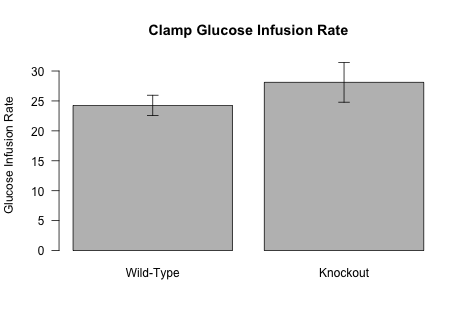
\includegraphics{figures/gir-1.png}

\subsection{Glucose Turnover}\label{glucose-turnover}

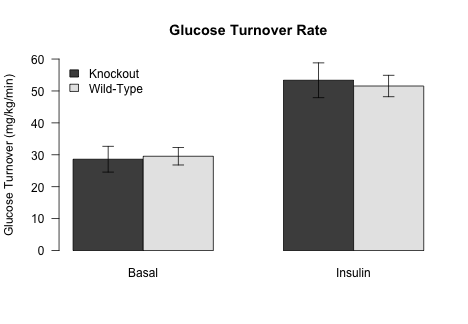
\includegraphics{figures/glucose-turnover-1.png}

\subsection{Endogenous Glucose
Production}\label{endogenous-glucose-production}

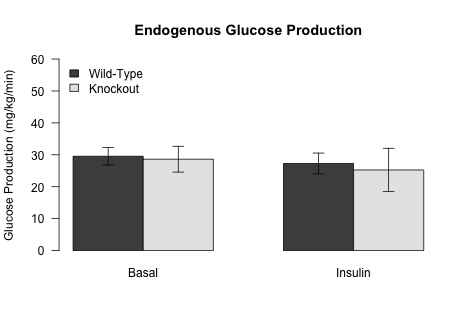
\includegraphics{figures/glucose-production-1.png}

\subsection{Clamp Summary}\label{clamp-summary}

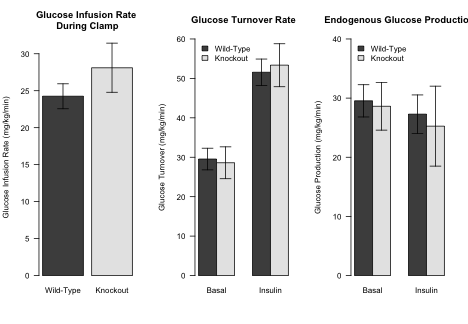
\includegraphics{figures/clamp-summary-1.png}

\subsubsection{Suppression of Endogenous Glucose
Production}\label{suppression-of-endogenous-glucose-production}

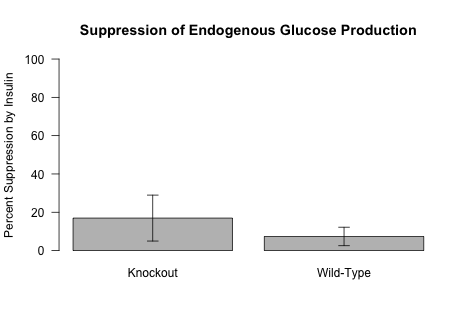
\includegraphics{figures/sHGP-1.png}

\subsection{Insulin Levels}\label{insulin-levels}

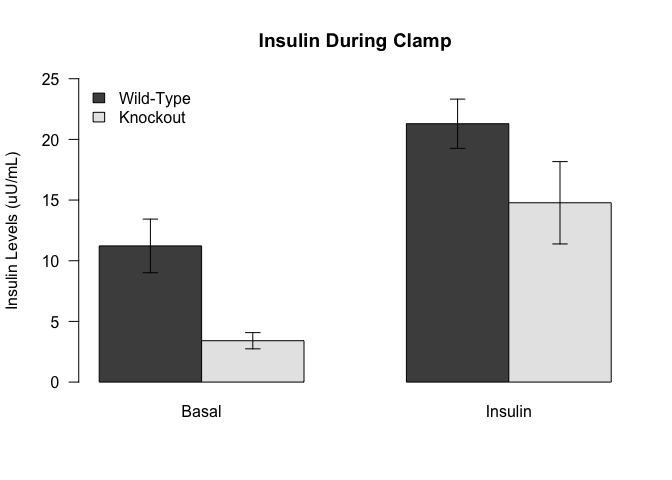
\includegraphics{figures/insulin-1.png}

\section{Glucose Clearance Rate}\label{glucose-clearance-rate}

Blood glucose clearance

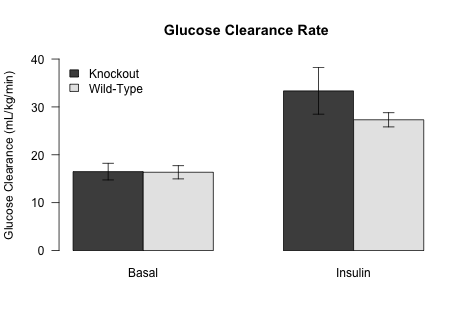
\includegraphics{figures/glucose-clearance-1.png}

\section{Tissue Glucose Clearance}\label{tissue-glucose-clearance}

\subsection{Gasctrocnemius Gluose Uptake During
Clamp}\label{gasctrocnemius-gluose-uptake-during-clamp}

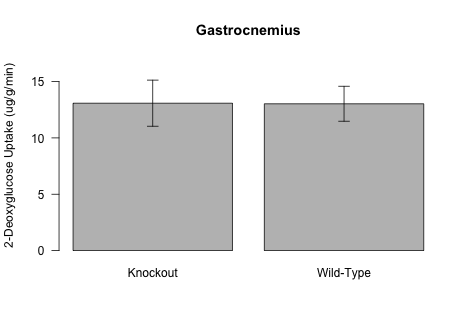
\includegraphics{figures/gastroc-1.png}

\subsection{Visceral Fat Gluose Uptake During
Clamp}\label{visceral-fat-gluose-uptake-during-clamp}

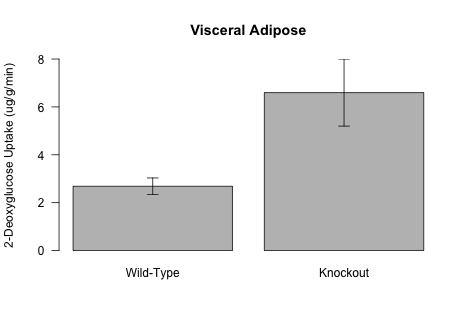
\includegraphics{figures/v-fat-1.png}

\subsection{Subcutaneous Fat Gluose Uptake During
Clamp}\label{subcutaneous-fat-gluose-uptake-during-clamp}

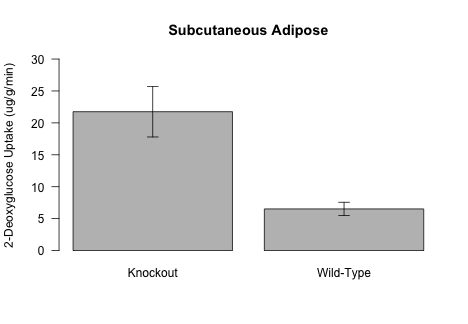
\includegraphics{figures/s-fat-1.png}

\subsection{Heart Gluose Uptake During
Clamp}\label{heart-gluose-uptake-during-clamp}

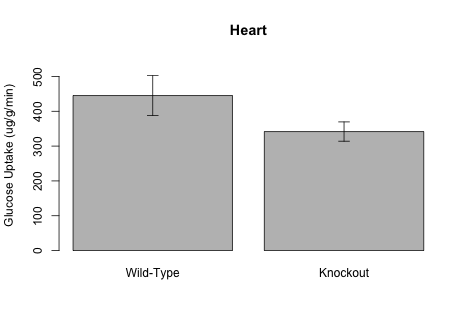
\includegraphics{figures/heart-1.png}

\subsection{Brown Adipose Tissue Gluose Uptake During
Clamp}\label{brown-adipose-tissue-gluose-uptake-during-clamp}

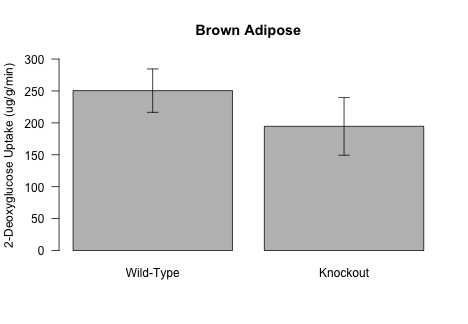
\includegraphics{figures/bat-1.png}

\subsection{Tissue Glucose Uptake
Summary}\label{tissue-glucose-uptake-summary}

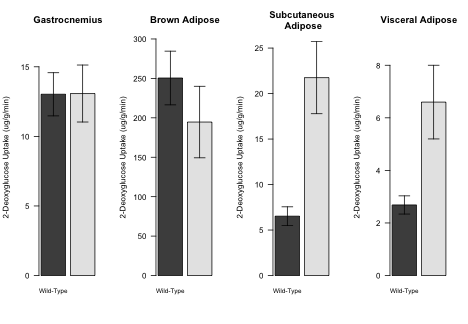
\includegraphics{figures/tissue-glucose-uptake-summary-1.png}

\section{Session Information}\label{session-information}

\begin{Shaded}
\begin{Highlighting}[]
\KeywordTok{sessionInfo}\NormalTok{()}
\end{Highlighting}
\end{Shaded}

\begin{verbatim}
## R version 3.5.0 (2018-04-23)
## Platform: x86_64-apple-darwin15.6.0 (64-bit)
## Running under: macOS  10.14.6
## 
## Matrix products: default
## BLAS: /Library/Frameworks/R.framework/Versions/3.5/Resources/lib/libRblas.0.dylib
## LAPACK: /Library/Frameworks/R.framework/Versions/3.5/Resources/lib/libRlapack.dylib
## 
## locale:
## [1] en_US.UTF-8/en_US.UTF-8/en_US.UTF-8/C/en_US.UTF-8/en_US.UTF-8
## 
## attached base packages:
## [1] stats     graphics  grDevices utils     datasets  methods   base     
## 
## other attached packages:
## [1] tibble_2.1.3     dplyr_0.8.3      tidyr_0.8.3.9000 knitr_1.23      
## 
## loaded via a namespace (and not attached):
##  [1] Rcpp_1.0.1       magrittr_1.5     tidyselect_0.2.5 R6_2.4.0        
##  [5] rlang_0.4.0      stringr_1.4.0    highr_0.8        tools_3.5.0     
##  [9] xfun_0.7         htmltools_0.3.6  yaml_2.2.0       digest_0.6.20   
## [13] assertthat_0.2.1 crayon_1.3.4     purrr_0.3.2      vctrs_0.2.0     
## [17] zeallot_0.1.0    glue_1.3.1       evaluate_0.14    rmarkdown_1.13  
## [21] stringi_1.4.3    compiler_3.5.0   pillar_1.4.2     backports_1.1.4 
## [25] pkgconfig_2.0.2
\end{verbatim}


\end{document}
